\documentclass[11pt]{article}
\usepackage{amsmath}
\usepackage{graphicx}
\usepackage[margin=0.5in]{geometry}
\author{Peter Lee}
\date{\today}
\title{Examination of gated networks within the Mackey-Glass time series}

\begin{document}
\maketitle

\section{Introduction}
A common application of recurrent neural network models is the
analysis patterns within time series. A specific
type of analysis is predictive forecasting, where one uses past
observations to predict those in the future. 

The Mackey-Glass (MG) \cite{MG} is known as a chaotic time series.
The MG sequence's chaotic behaviour when its parameters and initial
conditions enable it to undergo bifurcation makes it an interesting
for predictive forecasting, since it cannot be evaluated exactly
in generality. In the literature there has been many attempts for forecasting the MG
series. Lanedes et al. used a multi-layer perceptron with past control
points to calculate a non-linear approximation for forecasting future
points \cite{tr}. Farsa et al. used the same configuration as
\cite{tr} and with the validation of their NARX-Elman network showed
that there are many works that use the MG series as a way to validate
their models \cite{Farsa}.

In this paper I will be investigating how gated recurrent networks
compare to other recurrent and non-recurrent solutions for predictive
forecasting. More specifically, I will be investigating two types of
gated recurrent networks, Long Short term memory (LSTM) \cite{LSTM}
and Gated Recurrent Units (GRU) \cite{GRU} and comparing them to the
multi-layer perceptron (MLP) model, as developed by \ref{tr} and an
Elman (ELM) recurrent neural network.

Two experiments were conducted for predicting future MG values 1, 5,
10, and 30 steps ahead. The first is when the models fit to a single
MG series as did \cite{tr,}. The second is fitting models MG series with
free parameters to evaluate if the models could adapt to the shape of
the curve during evaluation. 

The first experiment showed little difference between the gated and
non-gated recurrent networks, regardless of parametric complexity. The
MLP performed similarly, as long the number of hidden nodes
remained low. Training for distant predictions did not cause much
increase in error (0.03 to 0.10) and also did not diverge the
models from each other in terms of performance. The second experiment showed that the MLP was unable to generalize to
having a randomized $\beta$. However, the performance between all the
recurrent networks remained similar. Although predicting distant
values increased error rates much more than the first experiment,
there was still little notable difference between the recurrent
models.

These predictive forecasting experiments showed that there seems to
little tangible benefit from using a gated network instead of an
ordinary Elman network. This suggests that
the gated network's structure to forget information may be
better suited for tasks that require active recall, like NLP tasks, or
calculating a single integrated value (Ktrans) , instead of ones like
predictive forecasting that can be acquired by analyzing slope. %I

\section{Models}
The MLP is a model that uses hidden non-linear
layers, as shown in equation (\ref{eq:MLP_h})
to approximate a function. RNNs are MLPs that use previous evaluations
of hidden nodes as input, forming recurrent connections. The most
simple RNN is the Elman network, with hidden nodes calculated in
equation (\ref{eq:RNN_h}).
Gated recurrent networks are networks that control the
amount of information that is held in hidden nodes between time
steps. With these gates, the model can selectively ``forget''
and ``focus'' on information. It is thought that their ability to select what information
passes to subsequent time steps is what enables them to perform so
well in various tasks \cite{}. The LSTM was one that was introduced in the early
2000's, while the GRU was introduced in 2012. It has been theorized
that the GRU is able to perform equally as well as the LSTM in many tasks. 
The hidden nodes for
LSTMs and GRUs are calculated by \ref{eq:LSTM_h} and \ref{eq:GRU_h}
respectively.

\begin{equation}
\mathbf{h} = f( W_xx+B)
\label{eq:MLP_h}
\end{equation}
\begin{equation}
\mathbf{h^t} = f(W_xx+W_hh^{t-1}+B)
\label{eq:RNN_h}
\end{equation}

%Fill in equations
\begin{equation}
\begin{split}
f^{t} = \sigma(W_{xf}x + W_{hf}h^{t-1}+B_f) \\
i^{t} = \sigma(W_{xi}x + W_{hi}h^{t-1}+B_i) \\
c`^{t } = \tanh(W_{xc}x+W_{hc}h^{t-1}+B_c) \\
c = c \circ f + i \circ c` \\
o= \tanh (W_{xo}x + W_{ho}h^{t-1} + B_o) \\
h^{t} = o \circ c  \\
\end{split}
   \label{eq:LSTM_h}
\end{equation}
\begin{equation}
\begin{split}
  z^{t} = \sigma(W_{xz}x + W_{sz}s^{t-1} + B_z) \\
  r^{t} = \sigma(W_{xr}x + W_{sr}s^{t-1} + B_r) \\
  h{t} = \tanh(W_{xh}x + W_{sh}s^{t-1} + B_h) \\
  s^{t} = (1-z) \circ h^{t} + z \circ s^{t-1} 
  \end{split}
  \label{eq:GRU_h}
\end{equation}
All these models were implemented in Tensorflow. Batch sizes of 1 were
used and AdamOptimizer \cite{adam} was used to train with learning rate
was set at $10^{-3}$. For predictive forecasting, the recurrent networks
were trained by predicting an entire future sequence with back propagation through
time. The MLP was trained by predicting future values using four
control points, $x(t), x(t-6), x(t-12), x(t-18)$, similar to \cite{tr}.

  \section {Experiments}
\subsection {Mackey-Glass Time Series}
MG series is modelled by the differential equation (\ref{eq:MG}).
\begin{equation}
  \begin{split}
\frac{dx(t)}{dt} = \frac{\beta x(t-\tau)}{1+x^n(t- \tau)} - \gamma x(t)\\
\tau,\beta,n,\gamma > 0
\label{eq:MG}
  \end{split}
\end{equation}
To generate the MG series, I used the Runge-Kutta (RK4) method to
integrate the differential equation, with a step size of
0.01. This implementation was realized in Python, using a queue
data-structure to recall the recurrent values. For training, only
$0<t<=500$ were used and similarly for testing 
$500<t<=1000$  were used, with $t \epsilon I$. The data vectors used
for input and labels were $X \epsilon x(t) $ and $ Y \epsilon x(t+t_0) \forall
t$. 

The forecasting task involves predicting $x(t+t_0)$, given previous
information $x(t), x(t-1) ... x(t)$. In general models for predictive forecasting
can be described by equation \ref{eq:pred_forecast}, with the goal of
choosing parameters, $\theta$ to minimize the error between $x(t+t_0)$
and $f$. In this case, I used mean squared error as the error function.
\begin{equation}
  x(t+t_0) \approx f(x(1);x(2);x(3)...x(t) | \theta)
  \label{eq:pred_forecast}
\end{equation}

\subsection{Experiments}
For each of the following
experiments, I
trained models with two layers of hidden nodes with sizes of 32, 64, 96, and 128 to
view the models with range of different hyper parameters and observe if
there was a trend in performance with increased complexity. For each
initialization I attempted forecasting with $t_0$ = 1, 5, 10, and 30,
to determine the degredation of performance with further forecasting.

%\subsection {Experiment 1: Constant MG Parameters}
The first experiment followed those of related works \cite{}, in that the
parameters of the MG series were kept constant to $\beta = 0.2$,
$\gamma = 0.1$, $\tau = 17$, and $n = 10$. The second experiment used 10 MG series with different
initializations of $0.1 < \beta < 4$ with a leave-one-out style
evaluation. For example, 9 different series were used as a training
set, while the last one was used as a training set. The motivation of
this experiment, which contrasts those of other authors, was to measure
how the well the recurrent models could adapt to the shape of the curve during
evaluation and essentially estimate the(se) randomized parameter(s).

\subsection{Evaluation}
To measure model performance, two metrics were selected. They are
the cumulative absolute difference (\ref{eq:cumabs}) and the
cumulative absolute difference of slopes
(\ref{eq:cumabsderiv}). The cumulative absolute difference, which is
equivalent to square root mean squared error, is used in the other
papers \cite{other}, and generally shows how far off each prediction
is from the truth. The cumulative absolute difference of slopes is
unique to this paper, and its purpose is to show whether a model can
adapt to sharp peaks in the functions, or whether the model just
generalizes to a smooth approximation of the curve.

%Xavier initialization
\begin{equation}
\label{eq:cumabs}
  \int_{t_{start}}^{t_{end}} | x(t) - p(t) |
\end{equation}
\begin{equation}
\label{eq:cumabs}
  \int_{t_{start}}^{t_{end}} | \frac{dx(t)}{dt} - \frac{dp(t)}{dt} |
\end{equation}

\section {Results}
\subsection {Experiment 1: Constant Parameters}
 Sample evaluations are presented
  in figure \ref{fig:func_evals}.  Note how the cumulative
   differences begin large and increase constantly throughout the evaluation.

 \begin{figure}
   \begin{center}
   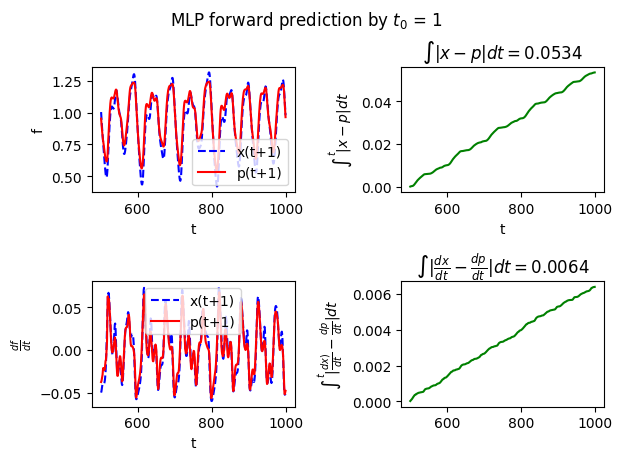
\includegraphics[width=.48\textwidth]{figures/MLP_1.png}
   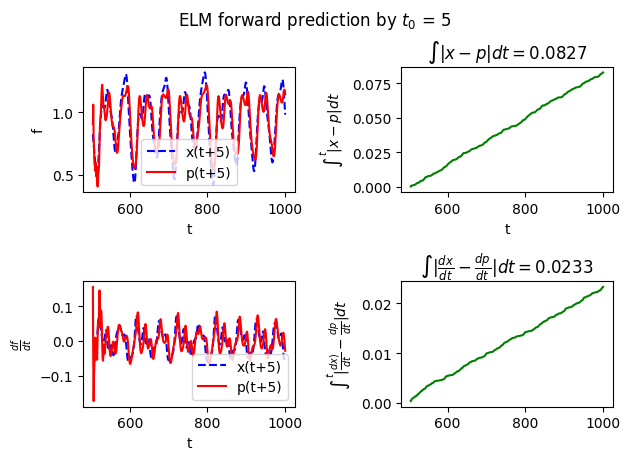
\includegraphics[width=.48\textwidth]{figures/ELM_5.png}
   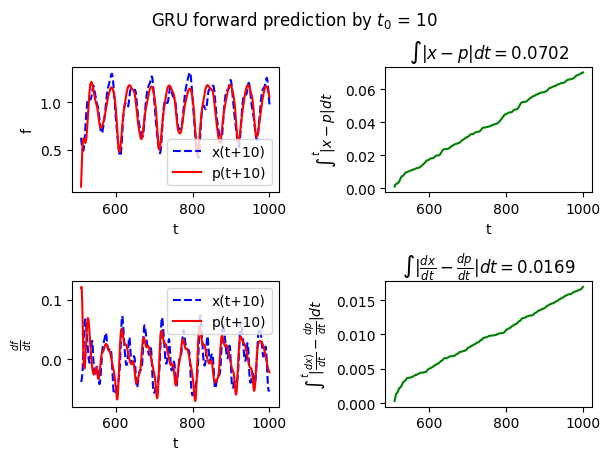
\includegraphics[width=.48\textwidth]{figures/GRU_10.png}
   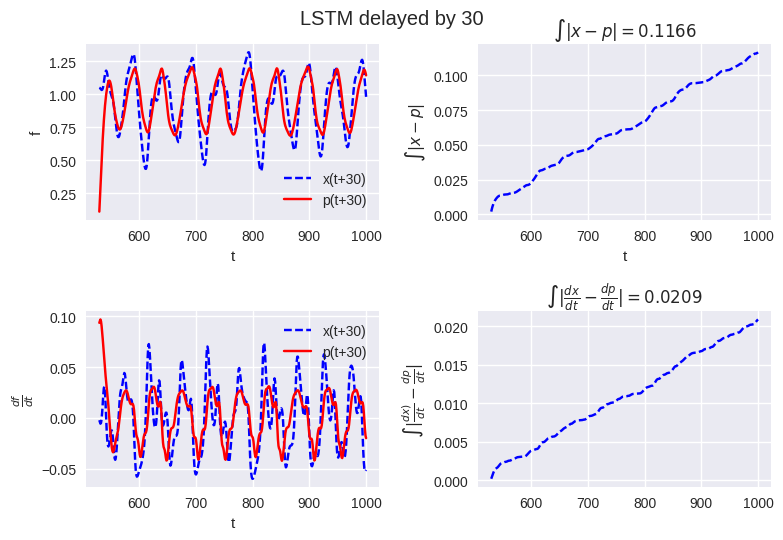
\includegraphics[width=.48\textwidth]{figures/LSTM_30.png}
 \end{center}
 \caption{Sample Curve fittings for MLP, ELM, GRU, and LSTM with
   delays of 1, 5, 10, and 30 respectively. The predicted and true
   values of the functions and slopes are plotted, along with the
   cumulative absolute differences.}
 \label{fig:func_evals}
   \end{figure}

  Figure \ref{fig:mg1_scatter} shows the performance of versions of models with
  respect to the number of parameters they possess**. It can be observed
  that all recurrent models seem to perform very similarly for $t_0 =
  1$. The MLP seems to fit well with less parameters, with overfitting
  likely occuring with an increased number of parameters, as shown 
  by the higher median and larger variance in (No
  regularization was attempted to keep models on par with each
  other). It seems that LSTM and GRU were scarcely effected by an
  increase in parameters. The ELM seems to perform slightly better
  then the other recurrent models, with the exception of $t_0 = 30$, where it seems to
  become more unstable. Overall all the models achieve similar
  performance in fitting to the static MG series. Since the recurrent
  models did not out perform the MLP, this raises the question as to
  whether fitting to a static MG series is the best benchmarking task
  for the MLP. %TOO long

  \begin{figure}
    \begin{center}
  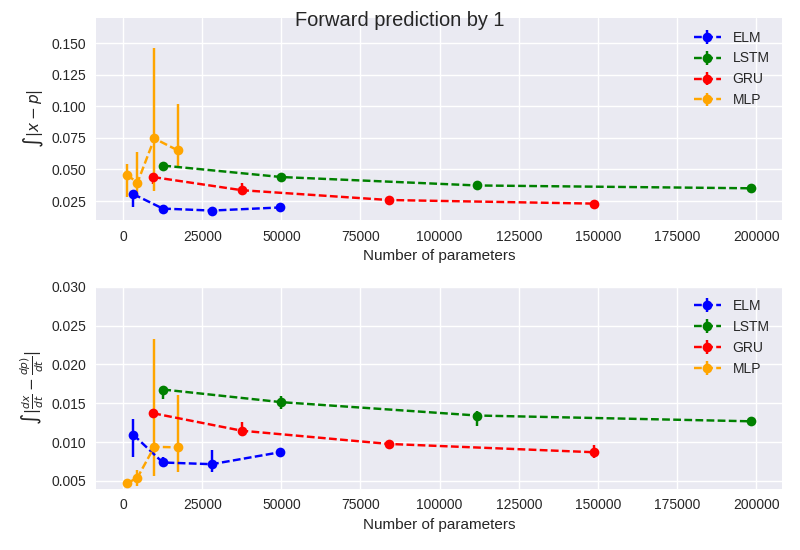
\includegraphics[width=.48\textwidth]{figures/mg1_scatter_1.png}
  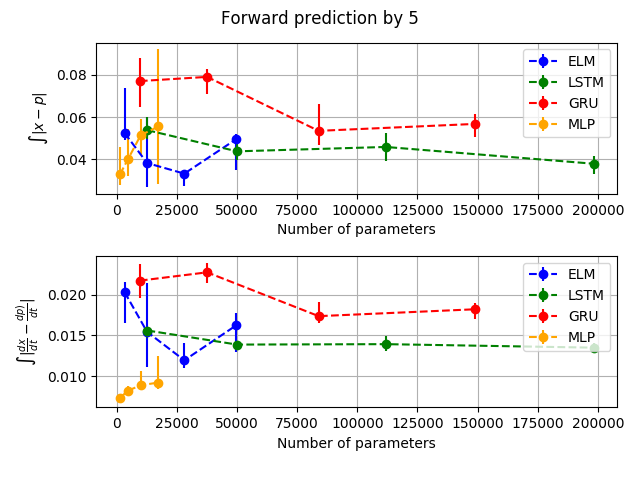
\includegraphics[width=.48\textwidth]{figures/mg1_scatter_5.png}
  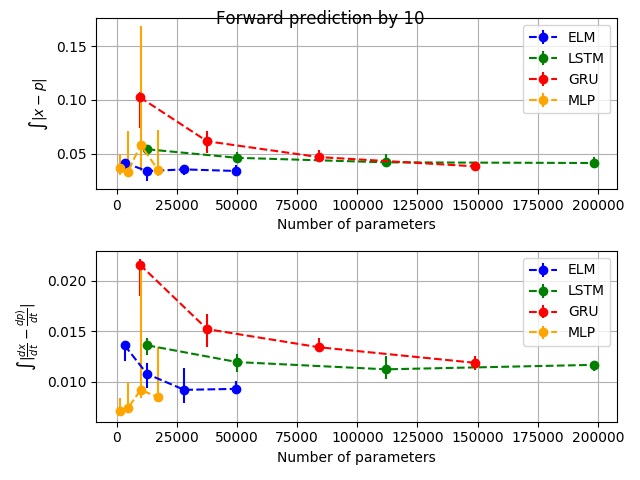
\includegraphics[width=.48\textwidth]{figures/mg1_scatter_10.png}
  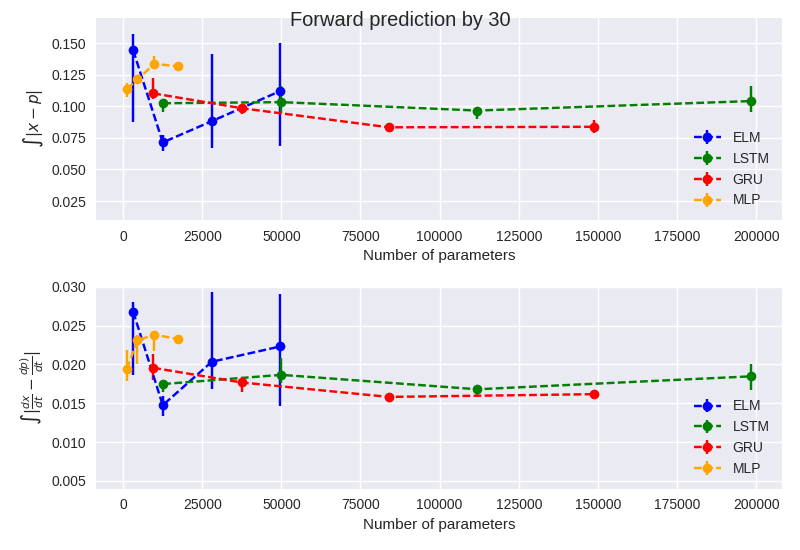
\includegraphics[width=.48\textwidth]{figures/mg1_scatter_30.png}
       
    \caption{Scatter plots showing model performance with respect to
      number of parameters. Using 10 evaluations with different weight
    initializations, points show the median with vertical bars
    extending 1 quartile above and below the median. From left to
    represent the models with hidden nodes of 32, 64, 96, and 128.}
    \label{fig:mg1_scatter}
    \end{center}
  \end{figure}

Alternatively figure \ref{fig:mg1_save} shows the performance of the models only
marginally reduced with longer term predictions. No model seems to
have an edge at producing predictions further in the future,
indicating that in static curve prediction, an MLP with control points
seem sufficient. This shows that 

  \begin{figure}
    \begin{center}
   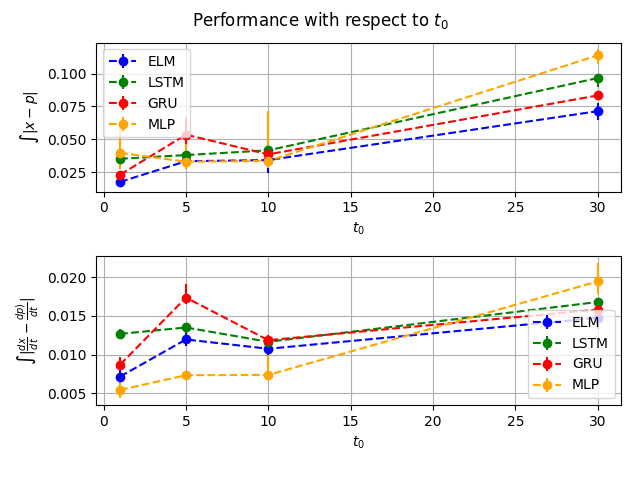
\includegraphics[width=.96\textwidth]{figures/mg1_save.png}
       
    \caption{Scatter plot showing the performance of models with 64 nodes
      per hidden layer as they are trained to predict values further
      in time.}
    \label{fig:mg1_save}
    \end{center}
  \end{figure}


 \subsection {Experiment 2: Randomized $\beta$}
Figure \ref{fig:mg2_func} shows sample evaluations for training with a
free parameter $\beta$. MLP was excluded from further analysis because
it became clear that it could not converge in this experiment. In this
case the cumulative metrics seem to have spike periodically in sync
with the peaks of the MG function. This seems to suggest that the
models have greater difficulty predicting large change in slopes than
in the previous experiment, with the predicted spikes occurring before
or after the actual point.

 \begin{figure}
   \begin{center}
   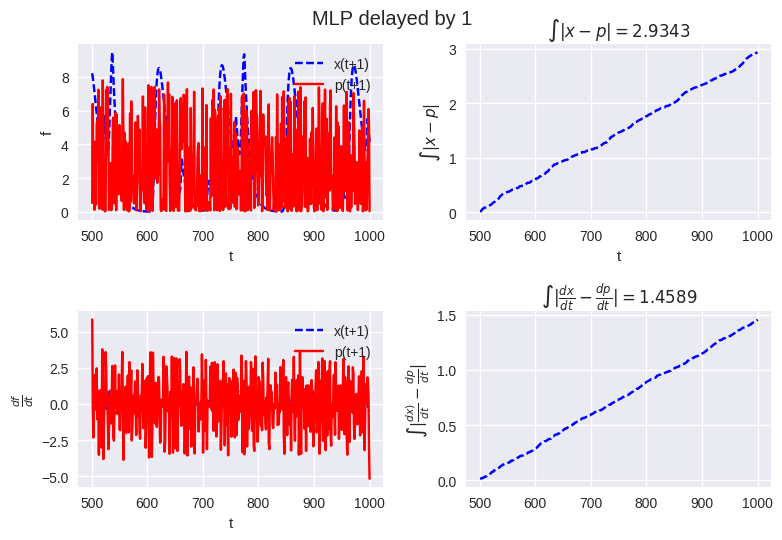
\includegraphics[width=.48\textwidth]{figures/MLP_1_mg2.png}
   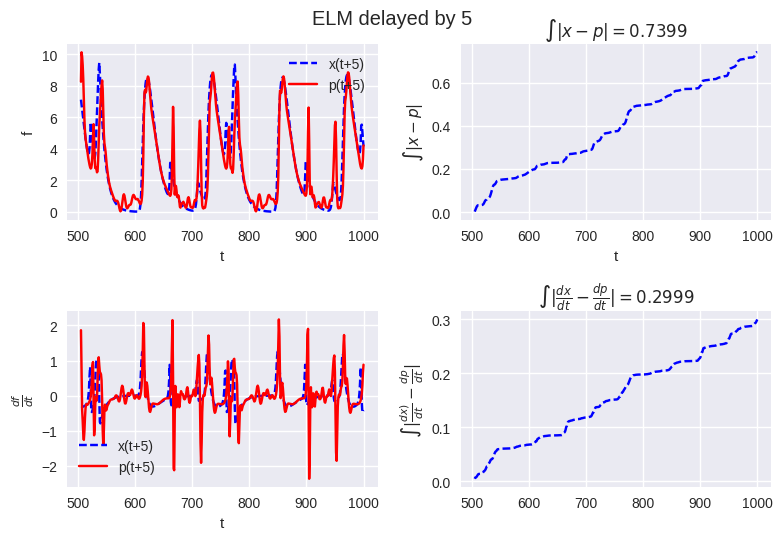
\includegraphics[width=.48\textwidth]{figures/ELM_5_mg2.png}
   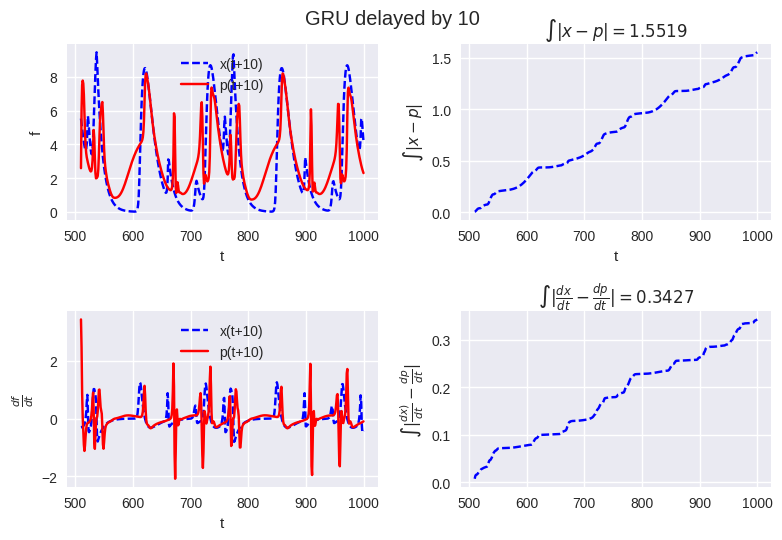
\includegraphics[width=.48\textwidth]{figures/GRU_10_mg2.png}
   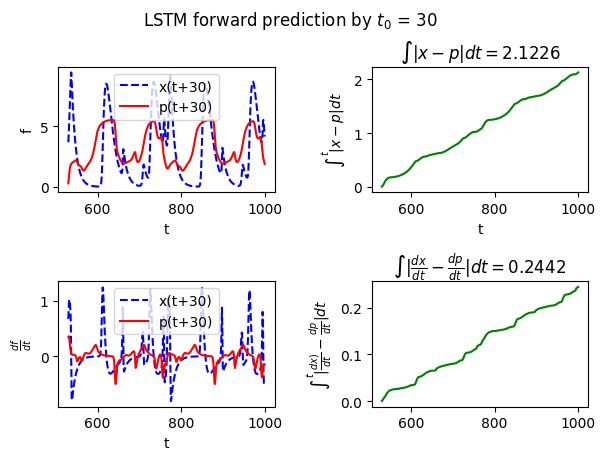
\includegraphics[width=.48\textwidth]{figures/LSTM_30_mg2.png}
 \end{center}
 \caption{Sample Curve fittings for MLP, ELM, GRU, and LSTM with
   delays of 1, 5, 10, and 30 respectively. The predicted and true
   values of the functions and slopes are plotted, along with the
   cumulative absolute differences.}
 \label{fig:mg2_func}
   \end{figure}

Figure \ref{fig:mg2_scatter} shows the performance of the models
compared with each other and the number of parameters they
suggest. There appears to be a slight improvement and stabilization
with more neurons similar to the last experiment. Similarly, there
does not seem to be any great disparity between any of the recurrent
models, showing how gated models may not be necessary for this task.

  \begin{figure}
    \begin{center}
  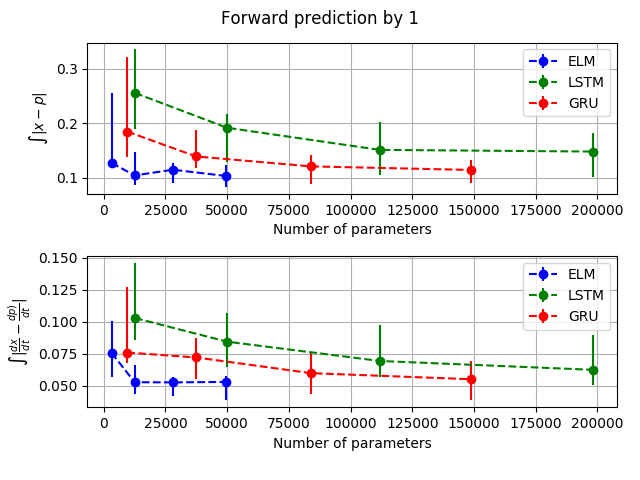
\includegraphics[width=.48\textwidth]{figures/mg2_scatter_1.png}
  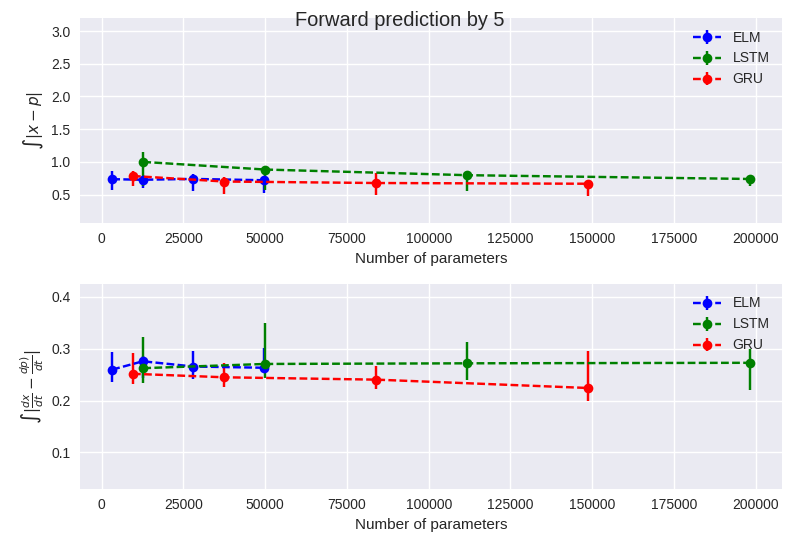
\includegraphics[width=.48\textwidth]{figures/mg2_scatter_5.png}
  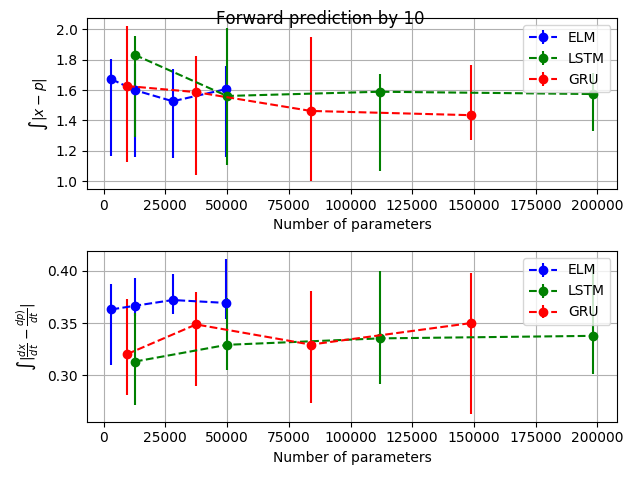
\includegraphics[width=.48\textwidth]{figures/mg2_scatter_10.png}
  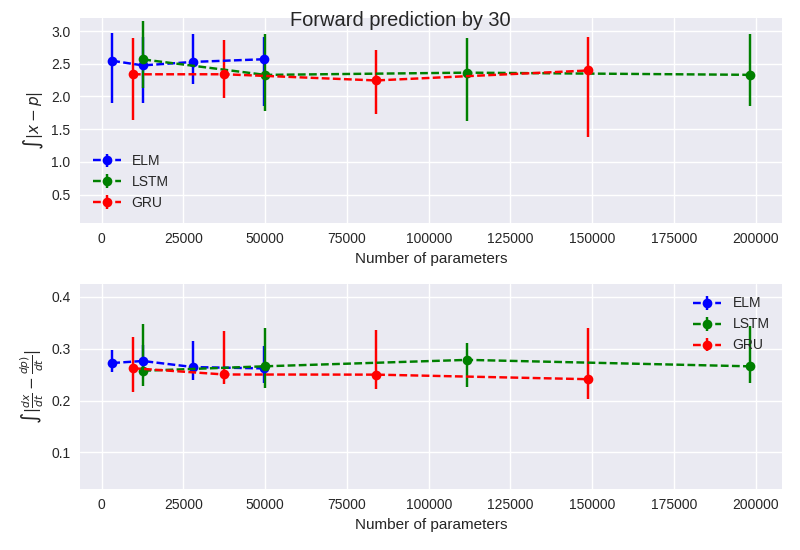
\includegraphics[width=.48\textwidth]{figures/mg2_scatter_30.png}
       
    \caption{Scatter plots showing model performance with respect to
      the number of parameters they possess in experiment 2. Conventions are the same as figure \ref{fig:mg1_scatter}.}
    \label{fig:mg2_scatter}
    \end{center}
  \end{figure}

In contrast to experiment 1, there seems to be a large degradation in
performance when the models are trained to predict further in the
future, as shown in figure \ref{mg2_save}. This is likely because the models cannot rely on a periodic
pattern in this case, but instead they need to take steps to
equivocally estimate the parameter and the shape of the curve. Again,
no model seems to have an edge at producing predictions further in the future. 

  \begin{figure}
    \begin{center}
   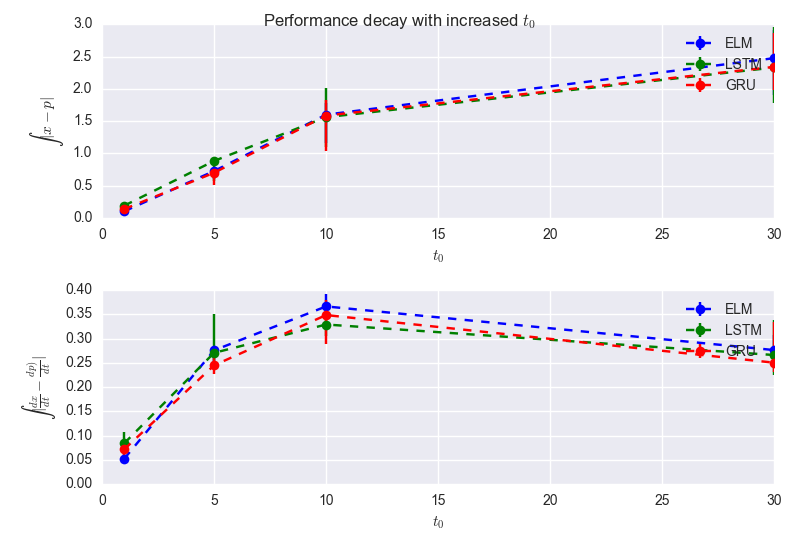
\includegraphics[width=.96\textwidth]{figures/mg2_save.png}      
    \caption{Scatter plot showing the performance of models with 64 nodes
      per hidden layer as they are trained to predict values further
      in time with a randomized $\beta$.}
    \label{fig:mg2_save}
    \end{center}
  \end{figure}

\section {Discussion}
It should be quite clear that the gated recurrent networks do not have
an advantage over the non-gated Elman network for this predictive
forecasting task. This could be because the ability to forget
information between time steps is less useful for this task, which
only requires extrapolating new points based on slope. In contrast,
tasks that requires discrete outcomes, such as NLP tasks, and those
that require integrating over the time series to provide a single
outcome may benefit more from the gated architecture. 

In terms of the limitations of this paper, it did not explore gated
networks with external memory (like the NARX network). Also, due to
time constraints, I was unable to perform experiments with other MG
parameters were randomized. This is unfornunate, as varying $\gamma$
may have yielded a more diverse effect than varying $\beta$, which
could have yielded different effects in the models. (Elman no gradient
peeking) (no regularization)

(Future work)

 \section{Conclusion}
I used the MG series to evaluate the performance of gated-recurrent
networks, the GRU and LSTM, against ELM and MLP networks. I created
two(three) experiments to test this: training with a MG series with
static parameters, and training with an MG series with its $\beta$
parameter randomized. The static experiment showed that all the models performed
equivalently.
It is curious why the static MG curve fitting is given as a benchmark
for so many time series analysis models, as it does test the ability
to adapt during evaluation of time series than my other
proposed experiments (rephrase to be correct), since it is clear that
the MLP can simply create a non-linear approximation. Varying $\beta$
(and $\gamma$) showed that the MLP was unable generalize with free
parameters. Also, there much larger reduction in accuracy for
predicting distant values, but nonetheless, there was little
difference between gated and non-gated RNNs in the large number
of configurations attempted.
% \appendices{}

\end{document}
